\tikzset{every picture/.style={line width=0.75pt}} %set default line width to 0.75pt        

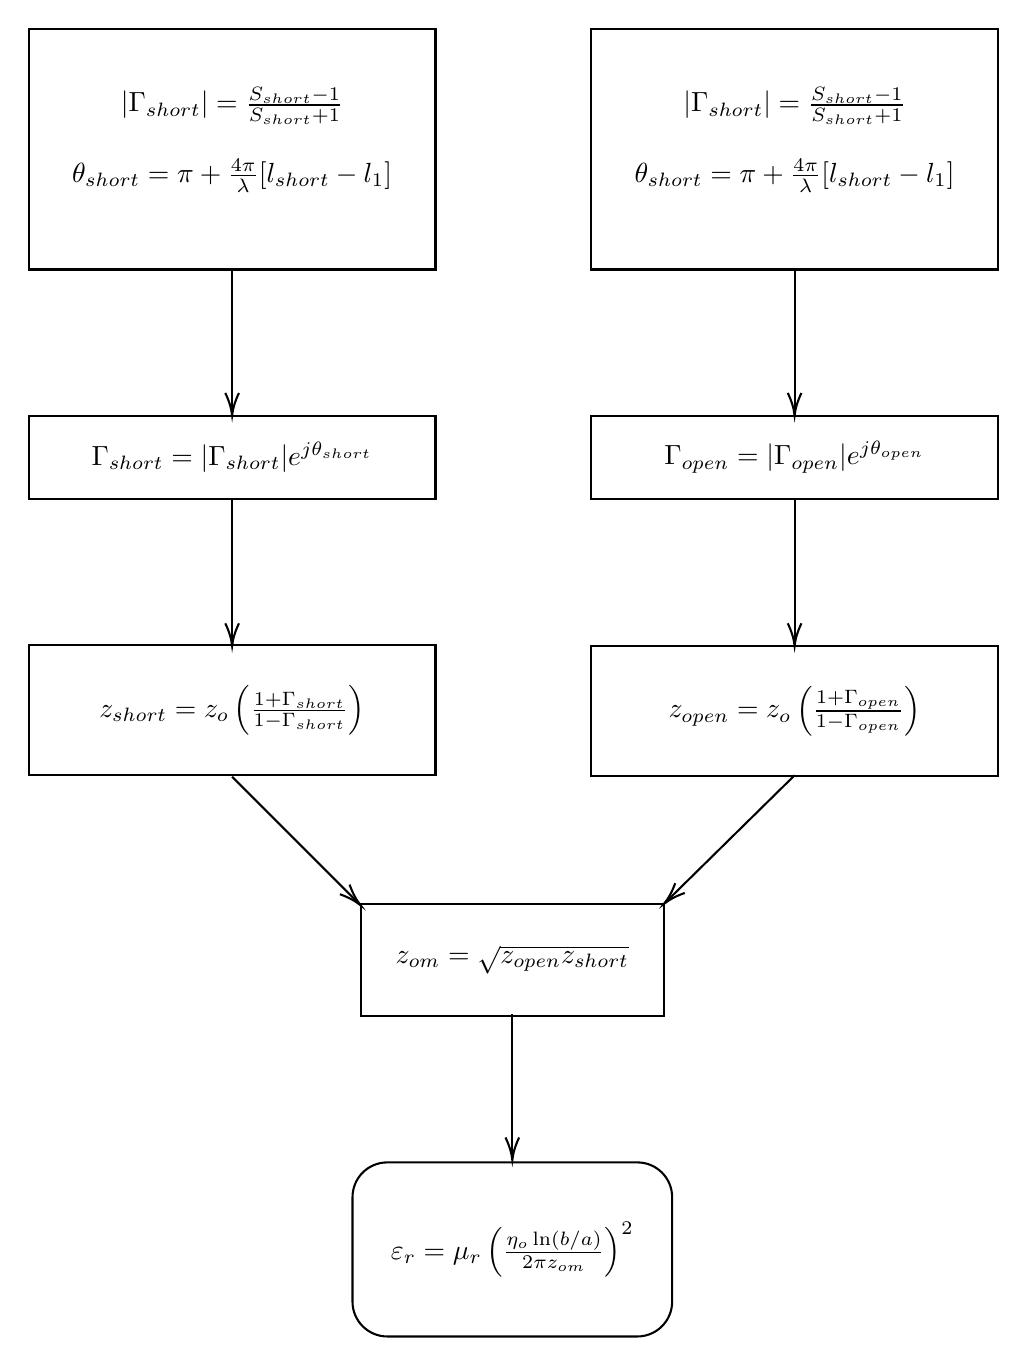
\begin{tikzpicture}[x=0.75pt,y=0.75pt,yscale=-1,xscale=1]
%uncomment if require: \path (0,657); %set diagram left start at 0, and has height of 657

%Shape: Rectangle [id:dp7126735491988057] 
\draw   (94,8) -- (290,8) -- (290,124) -- (94,124) -- cycle ;
%Shape: Rectangle [id:dp5768752679868709] 
\draw   (365,8) -- (561,8) -- (561,124) -- (365,124) -- cycle ;
%Straight Lines [id:da34420598529979385] 
\draw    (192,124) -- (192,192.42) ;
\draw [shift={(192,194.42)}, rotate = 270] [color={rgb, 255:red, 0; green, 0; blue, 0 }  ][line width=0.75]    (10.93,-3.29) .. controls (6.95,-1.4) and (3.31,-0.3) .. (0,0) .. controls (3.31,0.3) and (6.95,1.4) .. (10.93,3.29)   ;
%Straight Lines [id:da8417641803446987] 
\draw    (463,124) -- (463,192.42) ;
\draw [shift={(463,194.42)}, rotate = 270] [color={rgb, 255:red, 0; green, 0; blue, 0 }  ][line width=0.75]    (10.93,-3.29) .. controls (6.95,-1.4) and (3.31,-0.3) .. (0,0) .. controls (3.31,0.3) and (6.95,1.4) .. (10.93,3.29)   ;
%Shape: Rectangle [id:dp0887264533380483] 
\draw   (94,194.42) -- (290,194.42) -- (290,234.42) -- (94,234.42) -- cycle ;
%Shape: Rectangle [id:dp06732063654377773] 
\draw   (365,194.42) -- (561,194.42) -- (561,234.42) -- (365,234.42) -- cycle ;
%Straight Lines [id:da02670218063219898] 
\draw    (192,235) -- (192,303.42) ;
\draw [shift={(192,305.42)}, rotate = 270] [color={rgb, 255:red, 0; green, 0; blue, 0 }  ][line width=0.75]    (10.93,-3.29) .. controls (6.95,-1.4) and (3.31,-0.3) .. (0,0) .. controls (3.31,0.3) and (6.95,1.4) .. (10.93,3.29)   ;
%Straight Lines [id:da7673855623440871] 
\draw    (463,235) -- (463,303.42) ;
\draw [shift={(463,305.42)}, rotate = 270] [color={rgb, 255:red, 0; green, 0; blue, 0 }  ][line width=0.75]    (10.93,-3.29) .. controls (6.95,-1.4) and (3.31,-0.3) .. (0,0) .. controls (3.31,0.3) and (6.95,1.4) .. (10.93,3.29)   ;
%Shape: Rectangle [id:dp5668464351322218] 
\draw   (94,305.13) -- (290,305.13) -- (290,367.71) -- (94,367.71) -- cycle ;
%Shape: Rectangle [id:dp387927866207471] 
\draw   (365,305.42) -- (561,305.42) -- (561,368) -- (365,368) -- cycle ;
%Straight Lines [id:da24219615840965547] 
\draw    (463,367.71) -- (401.43,428.31) ;
\draw [shift={(400,429.71)}, rotate = 315.46] [color={rgb, 255:red, 0; green, 0; blue, 0 }  ][line width=0.75]    (10.93,-3.29) .. controls (6.95,-1.4) and (3.31,-0.3) .. (0,0) .. controls (3.31,0.3) and (6.95,1.4) .. (10.93,3.29)   ;
%Shape: Rectangle [id:dp3050012272660283] 
\draw   (254,429.71) -- (400,429.71) -- (400,483.71) -- (254,483.71) -- cycle ;
%Straight Lines [id:da5168465937110438] 
\draw    (192,368.42) -- (252.59,429.01) ;
\draw [shift={(254,430.42)}, rotate = 225] [color={rgb, 255:red, 0; green, 0; blue, 0 }  ][line width=0.75]    (10.93,-3.29) .. controls (6.95,-1.4) and (3.31,-0.3) .. (0,0) .. controls (3.31,0.3) and (6.95,1.4) .. (10.93,3.29)   ;
%Straight Lines [id:da14392593984104596] 
\draw    (327,482.71) -- (327,551.13) ;
\draw [shift={(327,553.13)}, rotate = 270] [color={rgb, 255:red, 0; green, 0; blue, 0 }  ][line width=0.75]    (10.93,-3.29) .. controls (6.95,-1.4) and (3.31,-0.3) .. (0,0) .. controls (3.31,0.3) and (6.95,1.4) .. (10.93,3.29)   ;
%Rounded Rect [id:dp28729239157386566] 
\draw   (250,570.97) .. controls (250,561.71) and (257.51,554.2) .. (266.77,554.2) -- (387.23,554.2) .. controls (396.49,554.2) and (404,561.71) .. (404,570.97) -- (404,621.29) .. controls (404,630.56) and (396.49,638.07) .. (387.23,638.07) -- (266.77,638.07) .. controls (257.51,638.07) and (250,630.56) .. (250,621.29) -- cycle ;

% Text Node
\draw (192,55.6) node [anchor=south] [inner sep=0.75pt]    {$|\Gamma _{short} |=\frac{S_{short} -1}{S_{short} +1}$};
% Text Node
\draw (192,69.4) node [anchor=north] [inner sep=0.75pt]    {$\theta _{short} =\pi +\frac{4\pi }{\lambda }[ l_{short} -l_{1}]$};
% Text Node
\draw (463,55.6) node [anchor=south] [inner sep=0.75pt]    {$|\Gamma _{short} |=\frac{S_{short} -1}{S_{short} +1}$};
% Text Node
\draw (463,69.4) node [anchor=north] [inner sep=0.75pt]    {$\theta _{short} =\pi +\frac{4\pi }{\lambda }[ l_{short} -l_{1}]$};
% Text Node
\draw (192,214.42) node    {$\Gamma _{short} =|\Gamma _{short} |e^{j\theta _{short}}$};
% Text Node
\draw (463,214.42) node    {$\Gamma _{open} =|\Gamma _{open} |e^{j\theta _{open}}$};
% Text Node
\draw (192,336.42) node    {$z_{short} =z_{o}\left(\frac{1+\Gamma _{short}}{1-\Gamma _{short}}\right)$};
% Text Node
\draw (463,336.71) node    {$z_{open} =z_{o}\left(\frac{1+\Gamma _{open}}{1-\Gamma _{open}}\right)$};
% Text Node
\draw (327,456.71) node    {$z_{om} =\sqrt{z_{open} z_{short}}$};
% Text Node
\draw (327,596.13) node    {$\varepsilon _{r} =\mu _{r}\left(\frac{\eta _{o}\ln( b/a)}{2\pi z_{om}}\right)^{2}$};


\end{tikzpicture}
